\documentclass[a4paper,12pt]{article}

\usepackage[english,brazil]{babel}
\usepackage[utf8]{inputenc}
\usepackage{icomma}
\usepackage{amsmath}
\usepackage{makecell}
\usepackage{graphicx}
\usepackage{fancyhdr}
\usepackage{url}
\renewcommand{\baselinestretch}{1.5}
\usepackage{titling}
\usepackage{geometry}
\usepackage{subfigure}
\geometry{
 a4paper,
 left=35mm,
 right=15mm,
 top=1in,
 bottom=1in,
}
\usepackage{amsmath}
\usepackage{amssymb}
\usepackage{subfigure}
\usepackage{multirow}
\usepackage[table]{xcolor}
\usepackage[backend=bibtex,style=ieee,sorting=none]{biblatex}
\usepackage{algorithm}
\usepackage[noend]{algpseudocode}
\usepackage{pdfpages}
\usepackage{enumerate}
\bibliography{main}
\newcolumntype{C}{>{\centering\arraybackslash}p{1em}}


\newpage

\begin{document}
\selectlanguage{brazil}

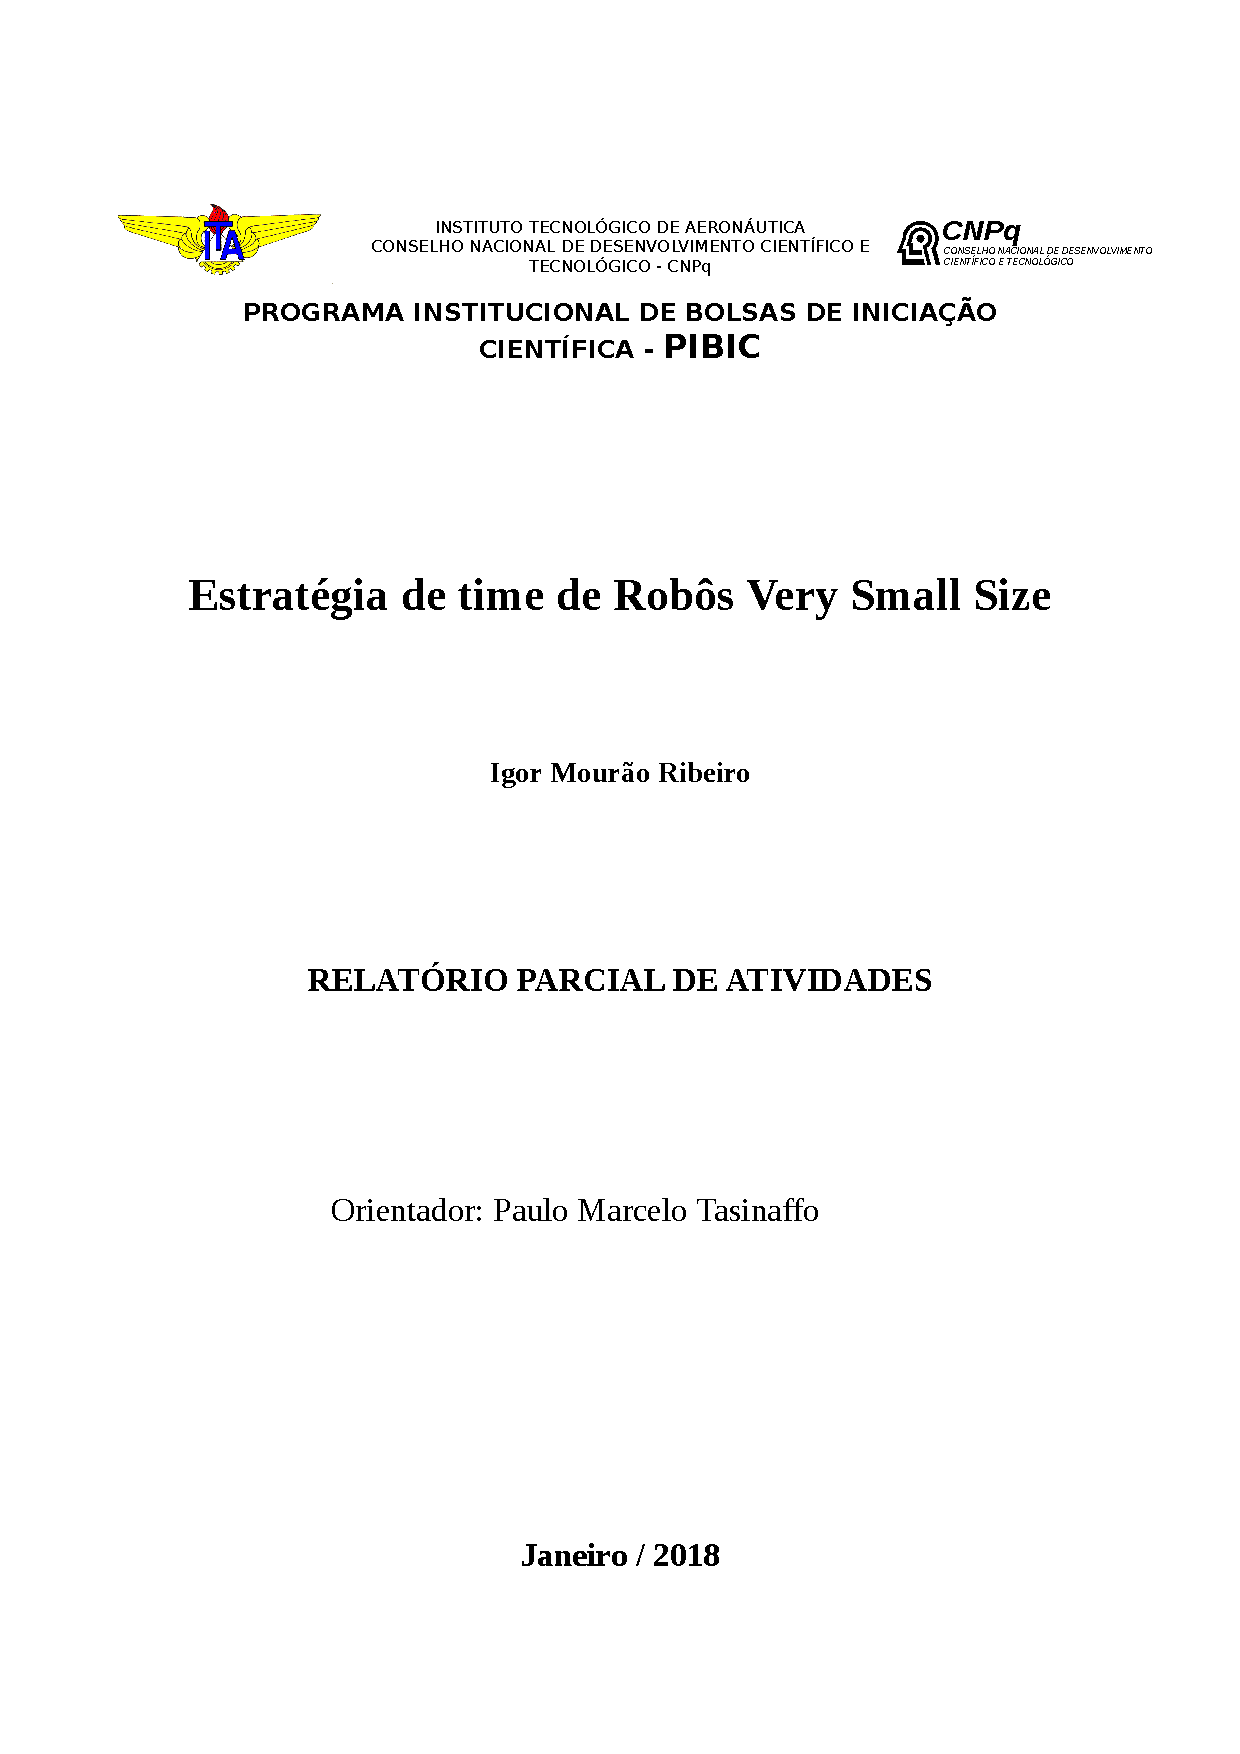
\includepdf[pages={1-},scale=1]{Inicio.pdf}


\tableofcontents

\newpage

\section{Resumo do Plano Inicial}
\label{secao:plano_inicial}

O objetivo deste trabalho é desenvolver e implementar um algoritmo para a estratégia de um time composto por três robôs diferenciais. O contexto é uma partida de futebol segundo a Competição Brasileira de Robótica (CBR), categoria IEEE Very Small Size Soccer (VSS). A partir da posição de cada robô, incluindo robôs oponentes, e da bola, deve-se obter a melhor ação que cada robô aliado deverá executar para que faça o maior número de gols no fim de uma partida considerando limitações mecânicas e de controle. Visa-se utilizar os algoritmos aqui implementados pela equipe da ITAndroids, que representa o ITA, na competição da Latin America Robotics Competition (LARC)/CBR de 2017 em diante.

Planejamento:
\begin{itemize}

\item 1o Bimestre (ago / set): Estudo da literatura e revisão bibliográfica sobre o tema de tomada de decisão para robôs jogadores de futebol.

\item 2o Bimestre (out / nov): Seleção de métodos a serem implementados para planejamento e codificação da implementação.

\item 3o Bimestre (dez / jan): Codificação de testes automatizados para comprovação da correta implementação do algoritmo. Redação do relatório parcial.

\item 4o Bimestre (fev / mar): Simulações computacionais de um partida completa para análise e adaptações do método em cenários realistas de futebol de robôs.

\item 5o Bimestre (abr / mai): Análise dos algoritmos implementados em termos de carga computacional e eficácia. Integração da estratégia com o restante do código.

\item 6o Bimestre (jun / jul): Redação do relatório final. Redação do artigo para o ENCITA. Teste final para o software completo no robô real, com todas as áreas do projeto operantes.

\end{itemize}

\section{Resumo das Atividades Realizadas}
\label{secao:atividades_realizadas}

Ao longo dos dois primeiros meses, foram realizados estudos e foi decidido que será usado o algoritmo Behavior Tree (Árvore de Comportamentos) para tomada de decisão. Esse algoritmo foi escolhido dentre de opções como Máquina de Estados Finita e Árvore de Decisões. Uma introdução a esses assuntos pode ser encontrada em Orozco~\cite{orozcomaquinas}, para máquina de estados finita, e em Russel e Norvig~\cite{decision_tree}, para Árvore de Decisões. Para uma descrição sobre a eficácia do algoritmo Behavior Tree (BT) no contexto da robótica, pode-se encontrar na referência \cite{behavior_tree_robotics}.

Ao longo do segundo e terceiro bimestres, a base do algoritmo foi implementada utilizando C++, que é a linguagem utilizada pela equipe. Foi, em seguida, realizada a codificação dos testes de unidade para os componentes principais do algoritmo, os nós intermediários da árvore. A performance computacional da BT foi analisada e mostrou resultados satisfatórios e condizentes com o que foi previsto. A estrutura básica do algoritmo estava pronta.

A parte da BT que considera as limitações de um robô real foi implementada e testada no time. 
O método  foi mostrado efetivo na LARC, ocorrida entre os dias 7 a 11 de novembro de 2017. O algoritmo mostrou que realiza troca de posições entre jogadores de forma fluida, de modo que a equipe tinha o posicionamento mais dinâmico da competição. A equipe da ITAndroids conquistou o sétimo lugar de 30.

\section{Descrição do Problema}
\label{secao:enunciado_problema}

No contexto do futebol de robôs, a tomada de decisão traz muitos desafios. A estratégia consiste no fato de se implementar um algoritmo que consiga utilizar o planejamento de trajetórias do robô da melhor maneira possível. Isso nos traz a um desafio de nível mais alto: decidir qual a melhor decisão que cada robô pode tomar em um certo momento considerando limitações de trajetórias possíveis de serem seguidas.

Nesse projeto, trabalhou-se com os robôs da competição IEEE Very Small Size (VSS): uma competição de futebol de robôs completamente automatizada em que cada robô tem como tamanho máximo um cubo de 7,5 cm de aresta. O campo de futebol possuil 1,5 m de comprimento e 1,3 m de largura. Cada time tem 3 jogadores: que podem assumir posições dinâmicas, como goleiro e atacante, ao decorrer de uma partida. Uma câmera proporciona a visão aérea com as posições de todos os elementos da partida. A visão computacional utilizada pela equipe ITAndroids pode ser encontrada com mais detalhes em \cite{tasinaffo_ic}. As regras completas podem ser lidas em \cite{cbr2008}.

\begin{figure}[H]
	\centering
	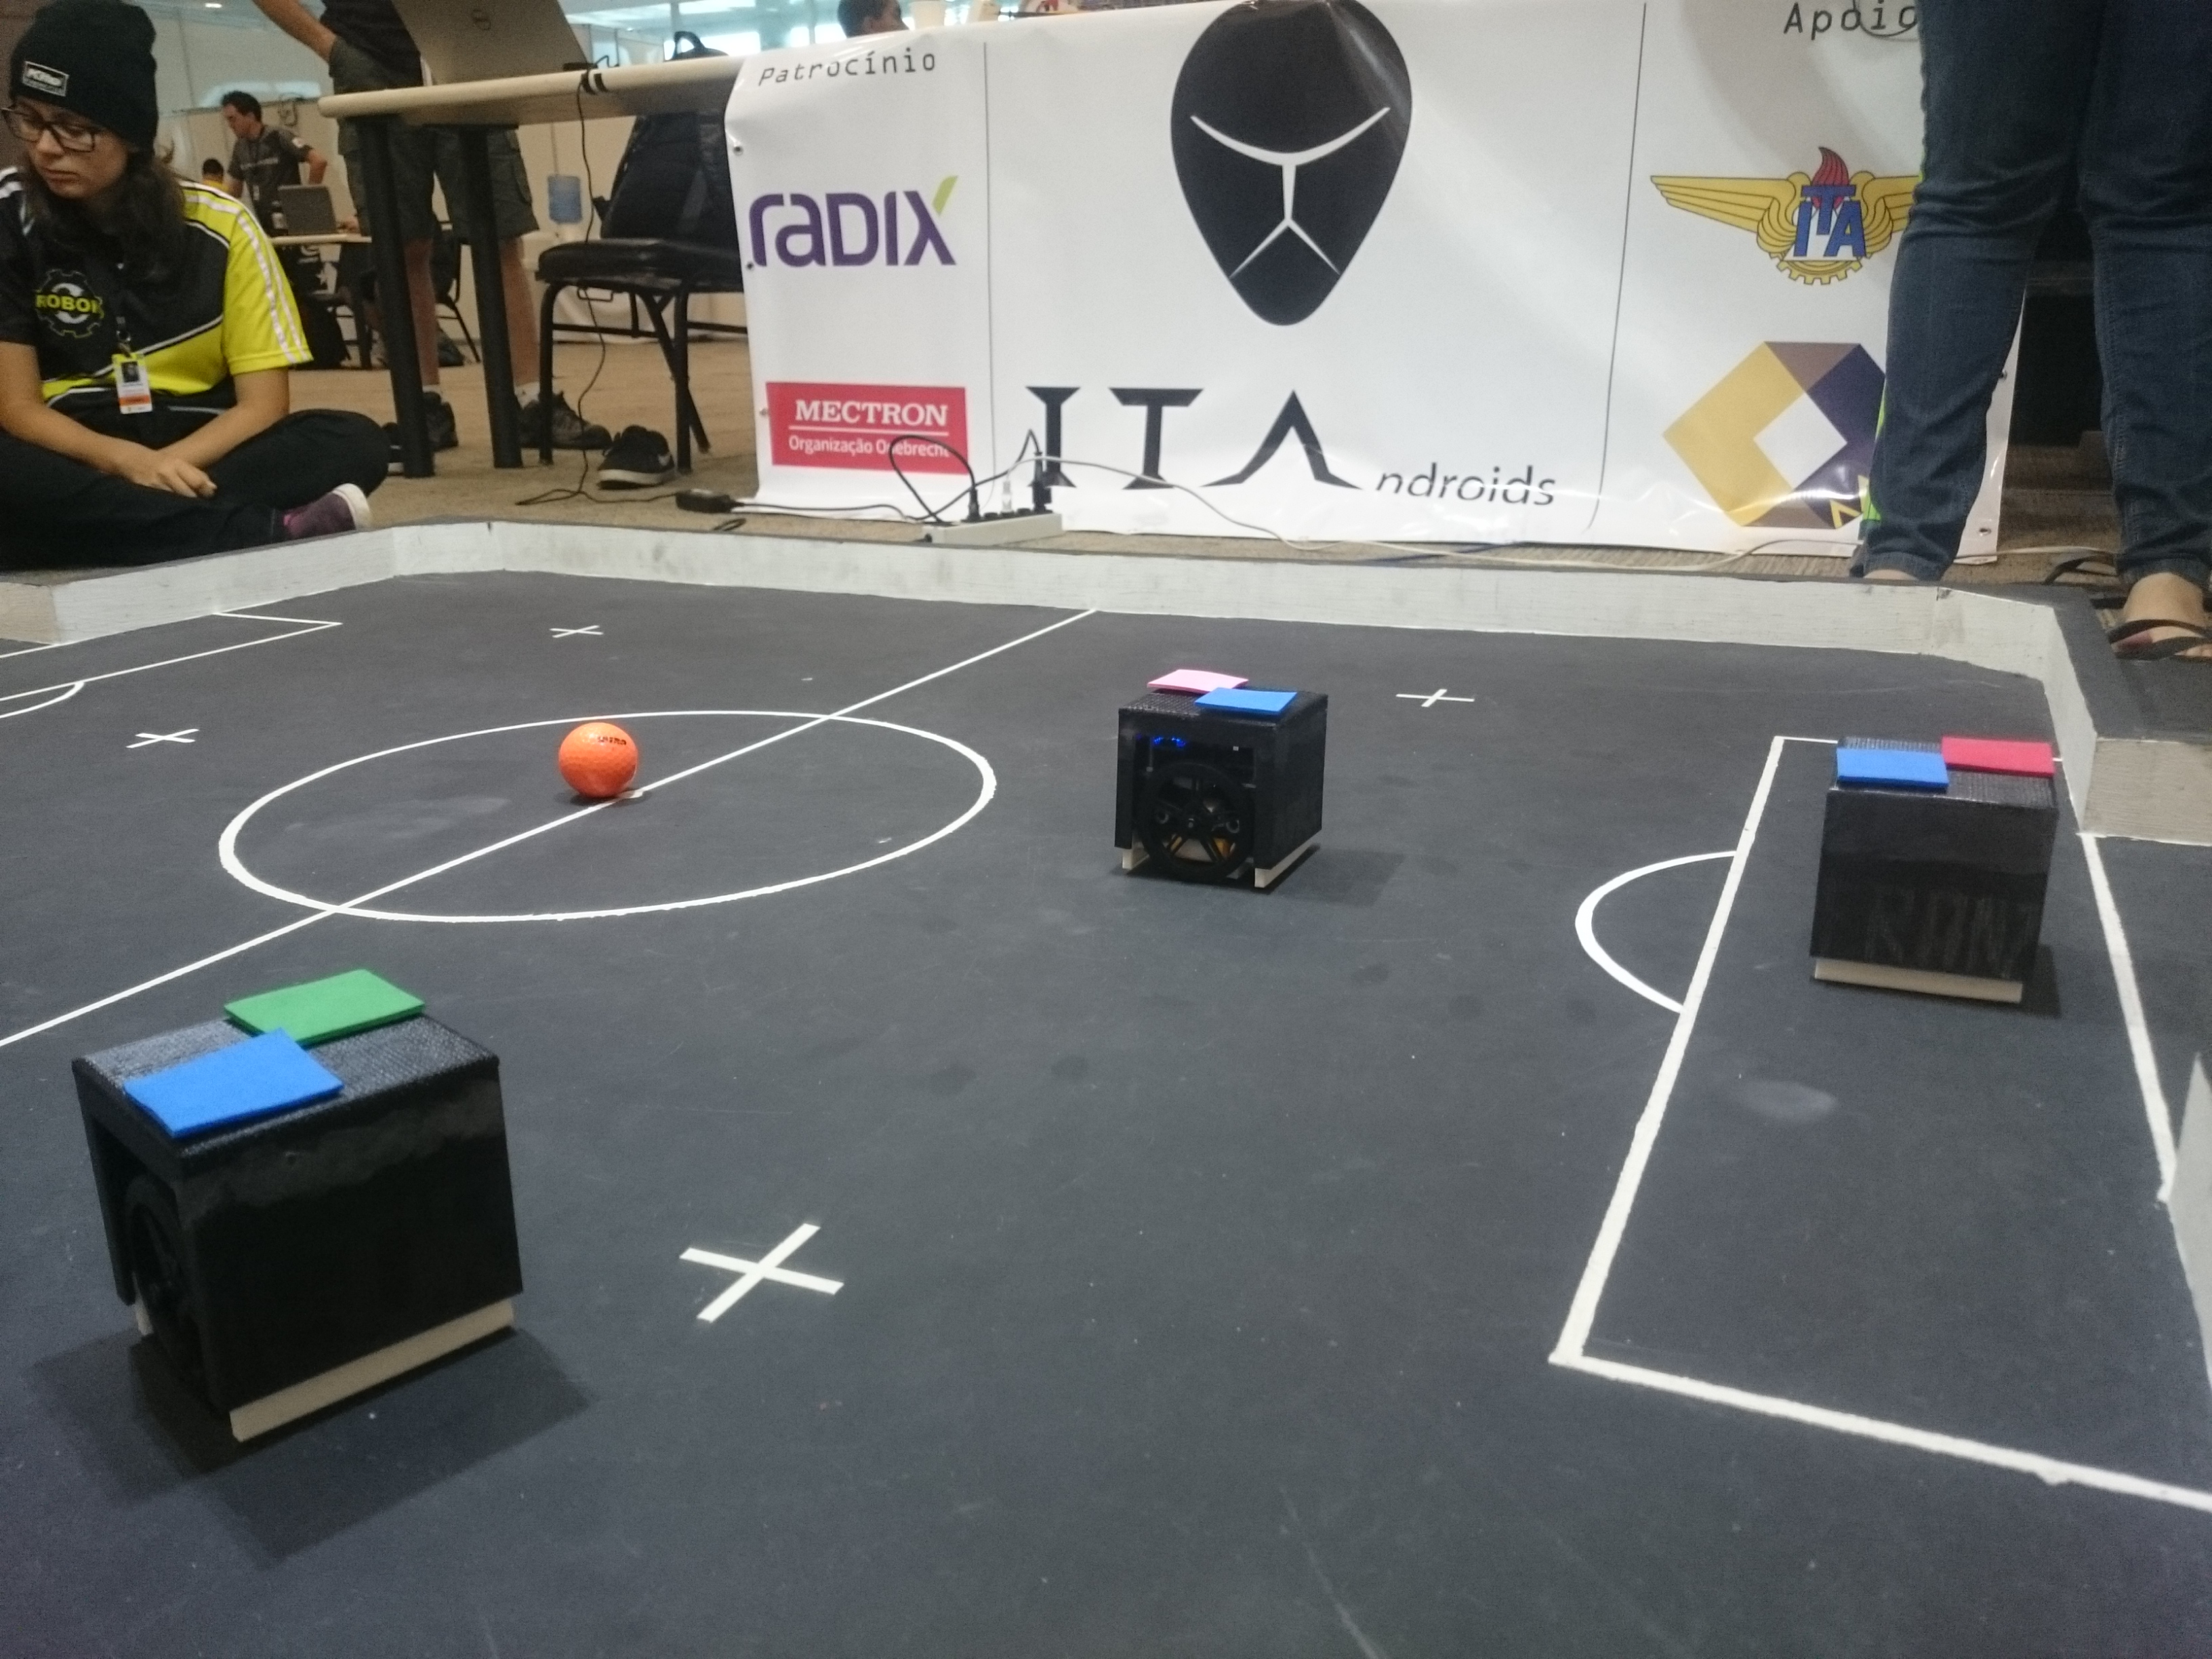
\includegraphics[width=0.5\textwidth]{figures/vss.JPG}
   \caption{Robôs da ITAndroids da categoria IEEE VSSS.} \label{fig:vss}
\end{figure}

A figura \ref{fig:vss} mostra os robôs usados nas competições. Cada robô foi projetado com duas rodas laterais e duas esferas livres à frente e atrás para manter o equilíbrio. Essa característica o torna um robô diferencial. Ou seja, temos o controle sobre as velocidades linear e angular, mas não é possível mover o robô para os lados. A linguagem utilizada para o projeto foi C++, pois é uma linguagem que tem uma velocidade de execução alta e tem escalabilidade descente para um projeto grande. 

Nesse contexto, surgem várias questões a serem resolvidas para se ter um time vencedor. Nesse projeto, será abordado o seguinte problema de estratégia: dada a posição e a velocidade de cada robô no campo, da bola e da direção que os nossos robores estão (não é possível descobrir a posição dos robôs oponentes, pois não sabemos a distribuição de cores que eles usam no seu topo), deve-se escolher qual posição o robô irá, com qual controlador  e qual planejamento de trajetórias utilizar. Deve-se também montar um plano para ações futuras, planejando uma sequência de posições que o robô deve ir para efetuar um gol.

O algoritmo de estratégia deve executar em tempo de execução de, no máximo, 16 ms para todo o time, que é o tempo de amostragem da câmera. A maior parte desse tempo é gasto com o planejamento de trajetórias usado, que é o Rapidly-exploring Random Tree (RRT). O tempo para cada execução de um RRT é de 1 ms, de acordo com \cite{franzoni_rrt}, limitando a em torno de um limite de doze chamadas do algoritmo por execução completa da estratégia, com uma margem de erro trinta e três porcento. Ressalta-se a importância de não ultrapassar esse tempo máximo, já que se isso acontecer perde-se uma imagem da câmera e o funcionamento do jogo é realizado de forma atrasado.

Deve-se, então, ser montado um esquema de posicionamento dinâmico em que não existam nem atacante, nem zagueiro, nem goleiro fixos, mas sim, uma ideia de que as posições dependam da posição de jogo, garantindo que os três jogadores possam estar mais bem posicionados e tenham liberdade para escolherem suas próximas ações.

Para resolver esse problema, foi escolhido como principal algoritmo para a tomada de decisão a Behavior Tree, embasado na decisão de um time referência no futebol de robô mundial na categoria Small Size League \cite{ssl}, the Near East University team: the NEUIslanders\cite{NEUIslanders_ssl}.


\subsection{Behavior tree}

Para se construir uma BT, é preciso primeiro entender o básico de sua estrutura. Uma BT é uma Árvore no sentido dado pela teoria dos grafos, como explicado em \cite{west2001introduction}. Por definição, cada nó dessa árvore será chamado de behavior.

Os nós de uma Behavior Tree são diferenciados em dois tipos: os nós folhas, que são os nós da árvore que não tem filhos e os nós compostos, que podem ter um ou mais filhos.

Todos os nós retornam, no final de sua execução, um dos três estados a seguir: TRUE, FALSE ou RUNNING, para indicar, respectivamente, que o nó foi terminado com sucesso, que foi terminado sem sucesso ou que o algoritmo deve executar esse nó por pelo menos mais uma iteração.

\subsubsection{Nó Folha}

Os nós folha são os nós terminais da Árvore e eles que representam as ações mais baixo níveis e concretas da estratégia. São divididas em dois tipos: nós de ação e nós condicionais.

\textbf{Nó de Ação} São os nós que de fato realizam uma ação, como se movimentar até a bola.

\textbf{Nó condicional} São nós que apenas retornam um estado sem realizar nenhuma ação concreta, como checar se o time está atacando.

\subsubsection{Nó composto}

Nós compostos são os nós intermediários da árvore, que  são resposáveis por escolher quais os nós que serão executados. São completamente reutilizáveis no sentido que apenas uma implementação de cada tipo de nó composto deve existir e ela poderá ser usada em diversas partes do código. Os principais tipos desses nós que foram usados para a estraegia estão listados a seguir:

\textbf{Selector Behavior} Nesse behavior, é selecionado um de seus filhos para ser acessado a seguir. Ele é usado quando tem-se várias maneiras de se realizar uma mesma ação e deve-se escolher a melhor delas em uma determinada situação. Ele funciona executando os filhos em uma determinada ordem e, assim que um dos filhos retorna TRUE ou RUNNING, esse nó retorna o mesmo valor. Se um filho retornar FALSE, o próximo filho será executado. Caso nenhum filho seja sucedido ou retorne que deve ser executado mais um vez, o nó retorna FALSE.

\textbf{Sequence Behavior} Esse nó executa cada um dos seus filhos em uma sequência bem definida e fixa. Ele é usado para fazer ações sequenciadas para completar um objetivo maior, por exemplo: chutar a bola para o gol oponente requer que o robô aliado esteja atrás da bola, o que significa que chegar atrás da bola e, em seguida, chutar a bola representam ações sequenciadas. Ele funciona de forma que, quando um filho retorna RUNNING ou FALSE, o behavior retorna o mesmo valor e, quando um filho retorna TRUE, ele avança para o próximo filho. Se todos os filhos retornarem TRUE, o behavior é bem sucedido e também retorna TRUE.

\textbf{Parallel Behavior} O objetivo desse nó é executar todos os seus filhos ao mesmo tempo, fato que pode ser obtido ao utilizar-se de processamento paralelo ou não. Se um filho retorna FALSE, o behavior retorna FALSE. Se todos os filhos retornarem TRUE, o behavior retorna TRUE. Em todas as outras situações, o behavior retorna RUNNING e continua sua execução por pelo menos outra iteração.

\textbf{Decorator} O nome para esse behavior é inspirado no conceito de Decorator em Software Design Pattern, que pode ser explicado em \cite{hunt2013gang}. No contexto da Behavior Tree, esse nó tem apenas um filho e ele modifica o comportamento do filho de alguma maneira. Um decorador pode ser diversos tipos, mas os mais usados no projeto foram 

\begin{enumerate}
\item AlwaysFail e AlwaysSucceed: que fazem que o fiho sempre retorne FALSE ou sempre retorna TRUE respectivamente.
\item UntilFail e UntilSucceed: fazem que o fiho sempre retorne RUNNING a não ser que ele retorna FALSE ou TRUE, respectivamente.
\item Invert: muda o retorno do filho de FALSE para TRUE e TRUE para FALSE.
\end{enumerate}


\subsection{Técnico}

Uma Behavior Tree, que embora consegue modelar comportamentos complexos com facilidade, nem sempre é a melhor escolha para determinadas situações. Por isso, a estratégia foi dividida em níveis de abstrações diferentes, em que a um Técnico, representado pela classe Coach, seria responsável por escolher e administrar quais árvore cada um dos três jogadores deveria usar no momento.
Com essa implementação, tem-se um agente externo controlando a função dos jogadores por meio da escolha de uma BT, que pode ser uma árvore para um goleiro, para um principal e para um auxiliar. Isso significa que, em um dterminado momento, o técnico pode escolher que o time tenha 1 goleiro, 1 principal e 1 auxiliar a até mesmo 3 principais ao mesmo tempo. Os requisitos esperados para cada um desses papéis será abortado a seguir. Além disso, também é função do técnico escolher o papel de cada jogador a cada iteração do código, de modo que as posições dos jogadores não sejam fixas ao decorrer do jogo.

\subsubsection{Goleiro} 

O goleiro é o jogador que deve ficar próximo ao gol aliado com o objetivo de proteger o gol de ataques oponentes. 
\begin{enumerate}
\item Ele deve ser capaz de defender bolas com velocidade lenta em direção ao gol, ao acompanham o movimento da bola seguindo a linha do gol. 
\item Essa posição deve conseguir proteger o gol de bolas rápidas, usando para isso um modelo de predição que supõe que a bola continuará em linha reta. Essa predição é necessária, pois, a altas velocidades, a taxa de amostragem da câmera não é alta o suficiente para conseguir comandar o robô apenas para seguir o movimento da bola, sendo necessário antecipar onde ela irá. A figura \ref{fig:goal_predict} mostra como essa predição linear funciona, indicando a direção da bola e o movimento que o goleiro deverá fazer para proteger o gol.

\begin{figure}[H]
	\centering
	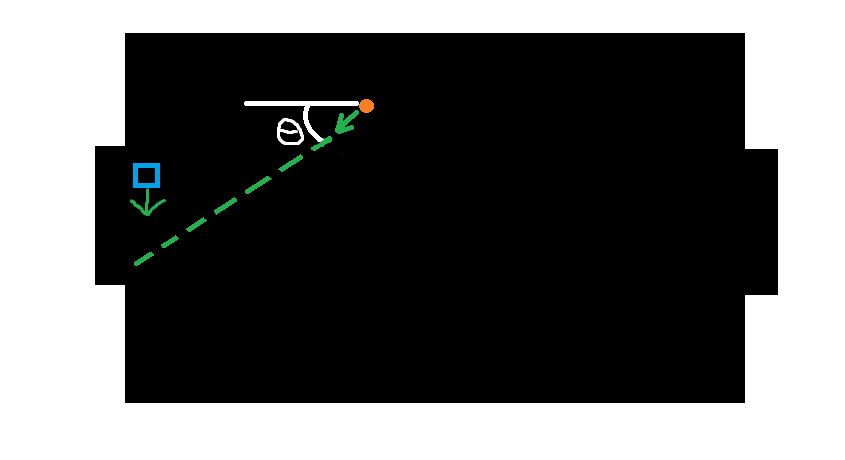
\includegraphics[width=0.8\textwidth]{figures/GoalierPredict.png}
   	\caption{Predição usada pelo goleiro para bolas rápidas.} \label{fig:goal_predict}
\end{figure}


\item Deve jogar a bola para longe do gol, por meio de rotações em torno do próprio eixo quando chegar próximo da bola para diminuir o risco de gol.
\item Deve sair do gol quando a situação não é de risco e ele chegará na bola antes de qualquer oponente. Nesse caso, outro jogador deverá se tornar um goleiro.
\end{enumerate}

\subsubsection{Principal} 

O jogador com o papel de Principal é o jogador mais ativo do time, que deve star constatemente avançando em direção a bola. Essa e o goleiro são as únicas posições que efetivamente deverao tocar na bola. Esse papel deve atender os seguintes requisitos:

\begin{enumerate}
\item deve atacar em direção ao gol oponente sempre que a bola não esteja muito próxima da parede. Isso será feito usando o planejamento de trajetórias RRT para se posicionar atrás da bola, seguido de uma rápida aceleração com a bola em linha reta em direção ao gol, de forma que o jogador leve a bola com a maior velocidade possível ao gol.
\item deve atacar pelas laterais do campo quando a bola estiver nos lados do campo de forma que ele jogue a bola para frente, sem necessariamente ter como objetivo fazer o gol, mas garantindo que o time agora esteja atacando. Para isso acontecer, será usado o RRT para se posicionar atrás da bola, seguida de uma rápida aceleração para frente.
\item deve girar em torno do próprio eixo quando estiver em um dos quatro cantos do campo. Caso esteja no ataque, esse giro fará que a bola se desloque para o meio do campo, o que pode significar que outro jogador possa pegar essa bola e levar para o gol, qualificando essa jogada com um passe entre jogadores. Caso a bola esteja em um dos cantos da defesa, o giro, além de tirar a bola da zona defensiva e a por numa posição de ataque, impedirá que a bola fique presa, fato que caracteriza em falta tiro livre segundo \cite{cbr2008}. A descrição da penalidade bola livre pode ser vista na imagem \ref{fig:bola_livre}.


\begin{figure}[H]
	\centering
	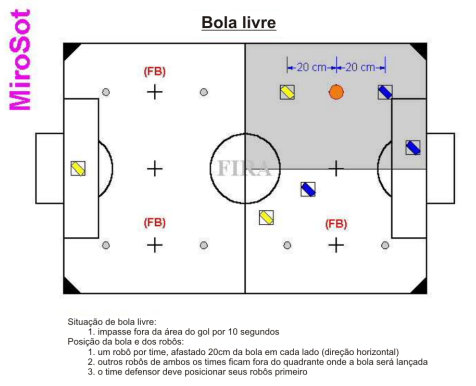
\includegraphics[width=0.8\textwidth]{figures/bola_livre.png}
   \caption{Descrição da penalidade bola livre.} \label{fig:bola_livre}
\end{figure}

 
\item deve ter comportamentos fixos e especiais para cada situações de falta, como por exemplo em um penalty, que ele deve levar a bola o mais rápido possível para um dos lados do gol para o goleiro não ter tempo de reagir e simplesmente atingir ou em um tiro livre, em que ele deve acelerar o máximo possível para chegar na bola antes do oponente. A descrição da falta do tipo penalty se encontra na figura \ref{fig:penalty}.

\begin{figure}[H]
	\centering
	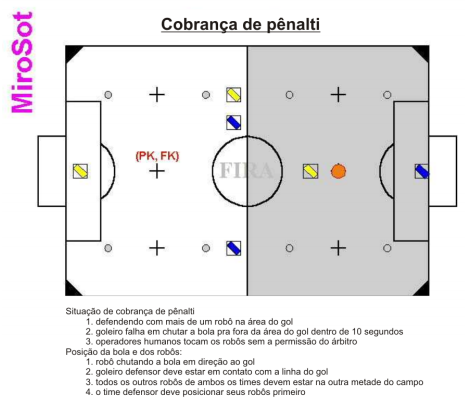
\includegraphics[width=0.8\textwidth]{figures/campo_penalty.png}
   \caption{Descrição da penalidade penalty.} \label{fig:penalty}
\end{figure}

\end{enumerate}




\subsubsection{Auxiliar} 

O auxiliar é um papél que tem apenas uma função: posicionar-se da melhor forma possível para manter um ataque consistente. A ideia é que, caso a situação seja oportuna, o auxiliar se torne o principal e comece a atacar a bola. Para escolher a posição que o auxiliar deverá ficar em uma determiada situação de jogo, foi utilizado a triangulação de Delaunay \cite{delaunay34} sobre o grafo de Voronoi \cite{voronoi08}. Esse algoritmo foi aplicado similarmente a \cite{akiyama2007multi}, relativo também à futebol de robôs.

Em seguida, uma interface foi desenvolvida para que fosse possível escolher as melhores posições dos jogadores aliados para cada posição da bola. A implementação para escolher a posição do auxiliar, no contexto da ITAndroids, funcionará seguindo os passos a seguir:

\begin{enumerate}

\item Escolhe-se uma posição estratégica para a bola no campo.

\item É escohido a melhor posição para um ou mais auxiliares quando a bola estiver nessa posição. A interface desenvolvida em C++, com a biblioteca Qt\cite{Qt}, foi usada para esses dois passos. A visualização pode ser vista na figura \ref{fig:delaunay_interface}.

\begin{figure}[H]
	\centering
	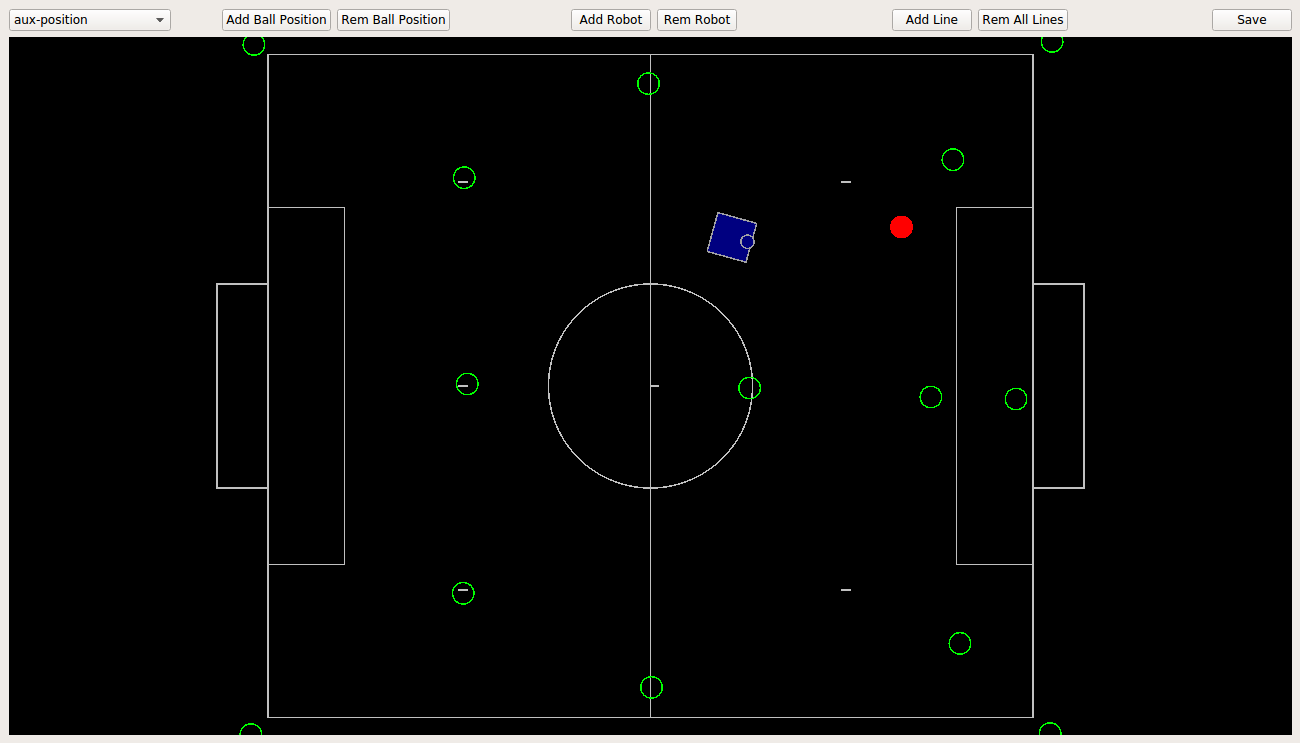
\includegraphics[width=1.05\textwidth]{figures/delaunay_interface.png}
   \caption{Interface para posicionamento com triangulação de Delaunay.} \label{fig:delaunay_interface}
\end{figure}

\item Os valores dessas posições são guardadas em um arquivos de texto para posterior uso no código da estratégia. Um exemplo desse arquivo de configuração se encontrar na figura \ref{fig:text_config_delaunay}, em que temos 2 jogadores em três posições, como escrito na linha 1 do arquivo; seguido pela localização da bola, com apenas as coordenadas x e y, e as posições dos jogadores, com as coordenadas x,y e ângulo. Essas localizações são repetidas três vezes conforme escolhido (linha 1).

\begin{figure}[H]
	\centering
	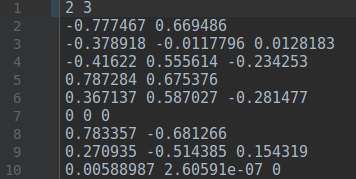
\includegraphics[width=0.8\textwidth]{figures/text_config_delaunay.png}
   \caption{Arquivo de configuração para posicionamento dcom triangulação de Delaunay.} \label{fig:text_config_delaunay}
\end{figure}

\item A estratégia do auxiliar utiliza a triangulação de Delaunay para a posição atual da bola, em conjunto com o arquivo de configuração feito, para interpolar as posições discretas escolhidas e fazer que o algoritmo retorna uma posição ótima independente da localização da bola.

\item Com a posição obtida pela triangulação, é usado o algoritmo de planejamento de trajetórias RRT, em conjunto com o seu controlador, para chegar nessa posição interpolada.

\end{enumerate}

\subsection{Táticas de Jogo}

Táticas de Jogo, representado pela classe 'Play', é a parte mais alto nível da estratégia. Essa classe é responsável por escolher qual técnico usar em um determinado momento da partida. O Play escolhe qual o melhor modo de se jogar em uma situação, como, por exemplo, ter uma postura mais agressiva ou mais defensiva envolvendo os três jogadores. Só pode existir um Play no jogo, que pode ser tratado como a raiz de uma Behavior Tree que tem os técnicos como filhos, tendo, cada um, três árvores relativas a cada jogador.

O seu funcionamento é similar ao Selector Behavior, no sentido em que é preciso escolher apenas um técnico a cada momento. Para avaliar quando é necessário fazer uma troca, usa-se o mesmo modelo de retorno: TRUE, FALSE e RUNNING para os técnicos. 

Dado essa troca, pode ser criados técnicos temporários para jogadas específicas de jogo, como o goleiro sair do gol e voltar outro jogador, que é uma ação de transição. Isso pode significar que um técnico principal pode chamar esse outro, voltando depois para o mesmo técnico novamente. Então, podemos ter um técnico principal e vários temporários para jogadas ensaidas e específicas que envolvam mais de um jogador.


\section{Resultados Obtidos}
	\label{secao: resultados_obtidos}
    
Nessa seção, são apresentados os resultados obtidos na resolução do problema da tomada de decisão para robôs jogadores de futebol IEEE Very Small Size Soccer.



Ao longo do primeiro bimestre, foi estudada a teoria necessária para se colocar o projeto em prática.
    
No início do trabalho, foi dedicado um mês para estudo de controle preditivo pelo livro \cite{maciejowski2002}, sendo adquirida uma base de conhecimento para nortear como deve ser a resposta do planejador de trajetórias. Não houve, a princípio, dificuldades na escolha dos métodos a serem utilizados. Os três algoritmos apresentados neste projeto foram escolhidos pelos seguintes critérios:

\begin{enumerate}
\item Campos potenciais já é largamente utilizado por equipes da competição IEEE Very Small Size. Em 2014, a ITAndroids tentou sua implementação, porém fracassou. O método foi assim escolhido por ser onipresente na competição e simples para a resolução deste problema.
\item RRT possui uma ampla gama de aplicações acadêmicas em robótica, sendo um método famoso. Em contraste com o anterior, ele é mais complexo e pode resolver o problema para casos mais genéricos: navegação por labirintos e por caminhos estreitos.
\item Otimização por MILP é um algoritmo que, em contraste com os anteriores, é menos empregado em estudos de robótica. Este método pode levar a resultados melhores que os anteriores, além de ser largamente explorado em diversos trabalhos de pesquisa recentes.
\end{enumerate}

Nos meses seguintes, até outubro, com o material passado pelo orientador, nas referências \cite{bellingham2002} e \cite{rubens2015}, foi estudado o método de otimização por MILP para navegação completa pelo mapa. A implementação foi feita em MATLAB, porém seu tempo de execução se mostrou muito longo e o método foi temporariamente descartado. Era necessária uma reformulação do algoritmo para simplificá-lo e torná-lo rápido o bastante.

Na primeira semana de outubro, foi implementado o método de campos potenciais em MATLAB e logo em seguida em C++. A fonte para os estudos foi o artigo \cite{khatib1986}. Foi realizado o teste para o ajuste de parâmetros e para a adaptação de casos especiais.

Nas duas semanas seguintes, prosseguiu-se para o estudo pelas fontes \cite{lavalle2011}, \cite{rubens2009} e \cite{howiechoset} e implementação do método RRT. As implementações em MATLAB e em C++ ficariam prontas ao final de outubro, sendo realizados os testes em cenário simplificado de forma que se pudesse ajustar as constantes e avaliar se o algoritmo seria aplicável ao robô real.

Nessa época, aproximava-se a competição da CBR 2015, sendo interrompida a série de testes do RRT. Foi escolhido o método de campos potenciais para ser utilizado pela ITAndroids. Na última semana de outubro e na primeira de novembro, ele foi testado no robô real. O ITA ganhou quarto lugar na categoria. Apesar do sucesso, foram encontrados vários erros durante os testes e algumas constantes tiveram de ser alteradas para a aplicação no evento. Após a competição, os testes do RRT em cenário simplificado foram concluídos ao longo do mês de novembro.

Durante o período de recesso (dezembro de 2015 a fevereiro de 2016), o método de otimização MILP foi reformulado com a divisão do campo na triangulação de Delaunay. Foi implementado em MATLAB, e nos dois meses seguintes (março e abril de 2016), foram realizados diversos testes em caso simplificado com o algoritmo afim de fazê-lo cumprir com os requisitos do problema. No entanto, os resultados não foram satisfatórios e, desta vez, o método foi definitivamente descartado.

No restante do tempo até a redação do relatório no mês de julho, foram realizadas simulações em cenários realistas para os dois primeiros métodos, sendo medidos os tempos e averiguando se os resultados se enquadram nos requisitos. Mais otimizações foram feitas para o RRT.

A seguir serão apresentados os resultados técnicos dos métodos de campos potenciais e de RRT para o seguinte cenário, com as simulações executadas em um computador com processador Intel Core i7 com \textit{clock} de $2,4 \, GHz$:

\begin{itemize}
\item Posição e direção iniciais, respectivamente: $(0;-0,6)$ e $\frac{1}{\sqrt[]{2}}(-1;1)$
\item Posição e direção finais, respectivamente: $(0;0,6)$ e $\frac{1}{\sqrt[]{2}}(-1;1)$
\item Obstáculos na posições: $(-0,3;0,3)$, $(-0,5;0)$, $(0,1;0)$ e $(0,5;-0,3)$
\end{itemize}
   
   
\begin{figure}[H]
	\centering
	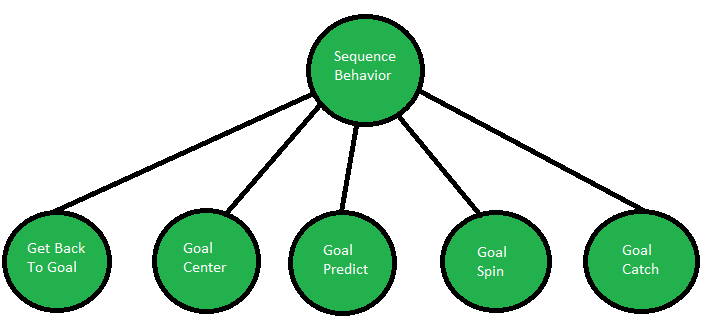
\includegraphics[width=0.8\textwidth]{figures/Goalier_BT.png}
   	\caption{Behavior Tree para o goleiro.} \label{fig:text_config_delaunay}
\end{figure}
   
\begin{figure}[H]
	\centering
	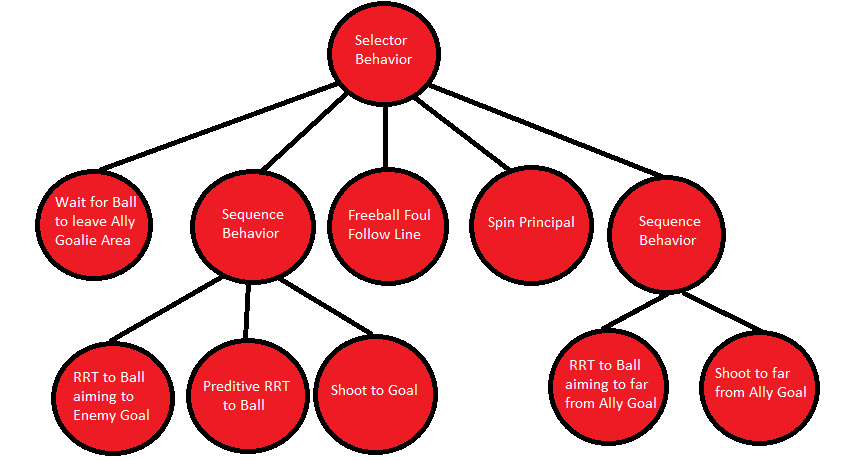
\includegraphics[width=0.8\textwidth]{figures/Principal_BT.png}
   	\caption{Behavior Tree para o principal.} \label{fig:text_config_delaunay}
\end{figure}   
   
\begin{figure}[H]
	\centering
	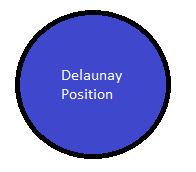
\includegraphics[width=0.4\textwidth]{figures/Auxiliar_BT.png}
   \caption{Behavior Tree para o auxiliar.} \label{fig:text_config_delaunay}
\end{figure}
   
   

   
   
\begin{figure}[H]
	\centering
	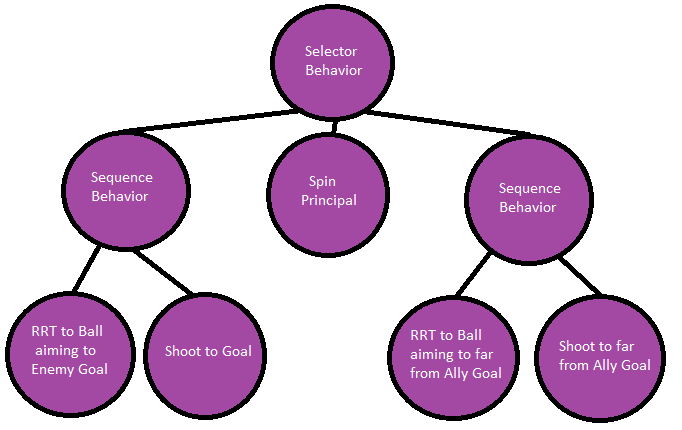
\includegraphics[width=0.8\textwidth]{figures/LastGoalierOutOfGoal.png}
   	\caption{Behavior Tree usada para o goleiro quando este sai do gol.} \label{fig:text_config_delaunay}
\end{figure}

   
   
\subsection{Campos potenciais}

\begin{figure}
\subfigure[Campos potenciais em MATLAB, trajetória não suavizada.]{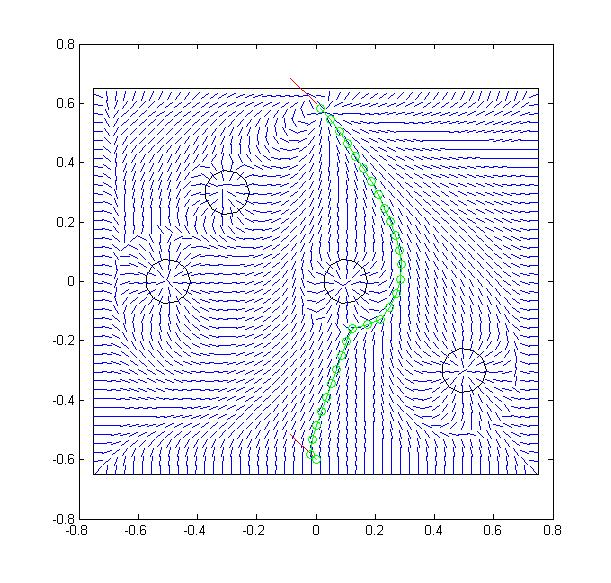
\includegraphics[width=0.47\textwidth]{figures/campospotML.jpg} \label{fig:sub:campospotML}}
\subfigure[Campos potenciais em C++, trajetória suavizada.]{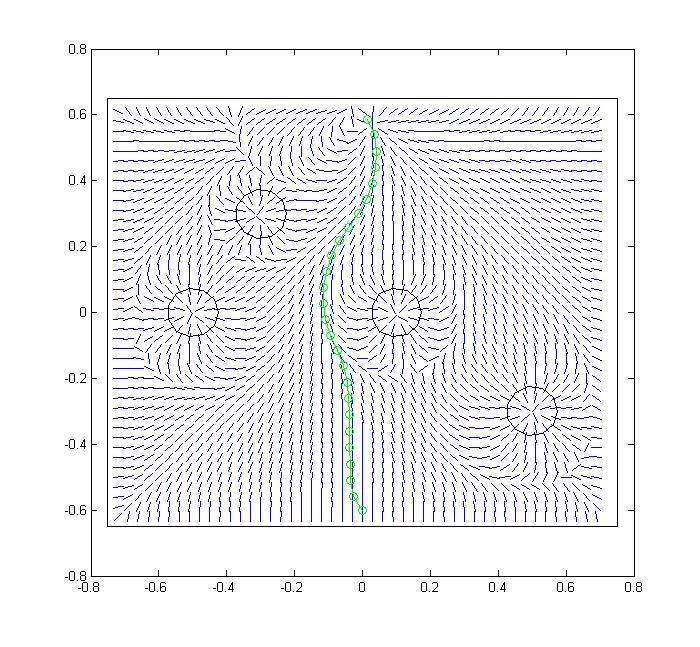
\includegraphics[width=0.47\textwidth]{figures/campospotC++.jpg} \label{fig:sub:campospotC++}}
\caption{Resultados com campos potenciais.}
\end{figure}
    
O algoritmo de campos potenciais foi testado primeiramente na plataforma MATLAB (Fig. \ref{fig:sub:campospotML}) para a configuração das linhas de campo. Em seguida houve o teste em C++ (Fig. \ref{fig:sub:campospotC++}). No primeiro, não foi utilizado o artifício de fazer o campo repulsivo do alvo decair para zero a partir de um limite. Foi observado que não há necessidade de se ter e efeito do dipolo elétrico em todo o espaço, pois o código em C++ gerou, neste teste e em outros, uma trajetória mais suave para o robô.

O tempo de execução foi excelente, sendo de apenas 0,0043 segundos em MATLAB. Em C++ a medição foi de 0,00098 segundos. Isso dá uma boa margem para o requisito de tempo de 2 ms para o planejador de trajetórias, o que o torna um candidato qualificado no quesito tempo.
    
\subsection{RRT}

O método foi testado em MATLAB (Fig. \ref{fig:rrtML}) e em C++ (Fig. \ref{fig:rrtC++}). No primeiro não foi implementada a suavização da trajetória. No segundo, sim.

\begin{figure}
\subfigure[RRT em MATLAB, trajetória não suavizada.]{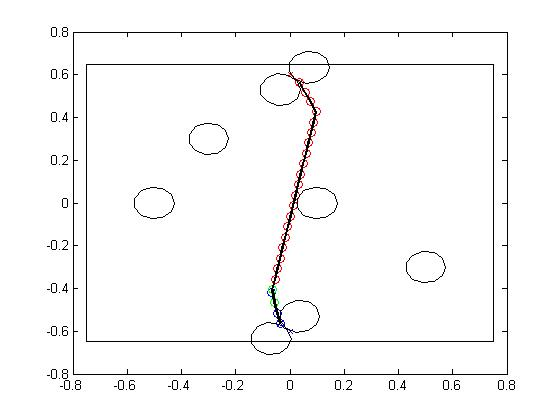
\includegraphics[width=0.47\textwidth]{figures/rrtML.jpg} \label{fig:rrtML}}
\subfigure[RRT em C++, trajetória suavizada.]{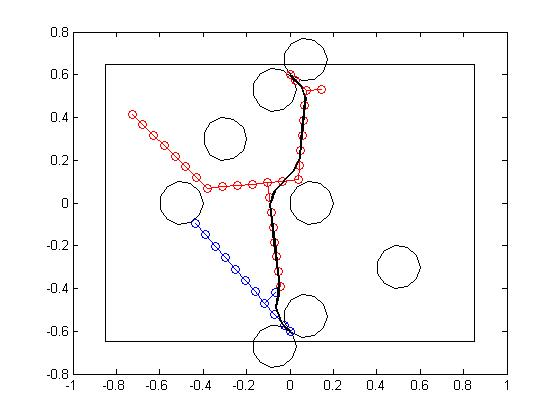
\includegraphics[width=0.47\textwidth]{figures/rrtC++.jpg} \label{fig:rrtC++}}
\caption{Resultados com RRT.}
\end{figure}

Sobre usar ou não usar a Quadtree, o parâmetro $h$ usado foi de $7$ $cm$, fazendo com que a média $n$ de nós das árvores seja da ordem de $50$. A diferença entre o tempo $O(\log{n})$ e $O(n)$ para a inserção, considerando que com o método simples não há alocação de memória e tampouco constantes altas, é pequena. A inserção $O(\log{n})$ com constantes é mais lenta que $O(1)$. O tempo com a Quadtree é aproximadamente o dobro em todos os testes realizados, sendo a estrutura, portanto, descartada.

Nesse caso, devido à característica aleatória do algoritmo, para evitar a variabilidade alta entre duas execuções consecutivas, buscando realmente se aproximar do ótimo, a trajetória é tomada como a melhor (menor comprimento) de um certo número de iterações do mesmo algoritmo. Para fazer a escolha do número de iterações para o algoritmo convergir para a solução ótima, da probabilidade $P$ e da $G$, foram realizados testes de forma a se obter as três tabelas de tempo, em milisegundos, nas tabelas da seção \ref{tab:Tempos_RRT_1}, respectivamente. Cada tempo é a média de $5000$ testes. Deve-se ter $P + G \leq 0,9$, pois deve haver pelo menos $0,1$ de probabilidade de se escolher um ponto aleatório no mapa.

\begin{table}[H]
\caption{Tempos de computação com 5 iterações - média de $5000$ ensaios.}
\centering{
  \begin{tabular}{|c|cccccccc|}
    \hline
    
	$G \backslash P$ & 0.0 & 0.1 & 0.2 & 0.3 & 0.4 & 0.5 & 0.6 & 0.7 \\ \hline
    0.0 & 0,723 & 0,610 & 0,586 & 0,578 & 0,601 & 0,621 & 0,672 & 0,760 \\
    0.1 & 0,804 & 0,621 & 0,599 & 0,608 & 0,642 & 0,683 & 0,761 & 0,939 \\
    0.2 & 0,878 & 0,641 & 0,633 & 0,647 & 0,697 & 0,786 & 0,986 & 1,488 \\
    0.3 & 0,846 & 0,676 & 0,681 & 0,709 & 0,817 & 1,006 & 1,565 & - \\
    0.4 & 1,046 & 0,758 & 0,788 & 0,854 & 1,030 & 1,697 & - & - \\
    0.5 & 1,059 & 0,809 & 0,866 & 1,041 & 1,624 & - & - & - \\
    
	\hline
  \end{tabular}
}
\label{tab:Tempos_RRT_1}
\end{table}

\begin{table}[H]
\caption{Tempos de computação com 10 iterações - média de $5000$ ensaios.}
\centering{
  \begin{tabular}{|c|cccccccc|}
    \hline
    
	$G \backslash P$ & 0.0 & 0.1 & 0.2 & 0.3 & 0.4 & 0.5 & 0.6 & 0.7 \\ \hline
    0.0 & 1,605 & 1,128 & 1,098 & 1,106 & 1,144 & 1,207 & 1,329 & 1,526 \\
    0.1 & 1,530 & 1,179 & 1,155 & 1,174 & 1,243 & 1,380 & 1,575 & 1,969 \\
    0.2 & 1,740 & 1,206 & 1,235 & 1,283 & 1,389 & 1,553 & 1,935 & 3,049 \\
    0.3 & 1,784 & 1,278 & 1,300 & 1,443 & 1,626 & 1,977 & 3,124 & - \\
    0.4 & 2,612 & 1,404 & 1,455 & 1,644 & 2,042 & 3,228 & - & - \\
    0.5 & 2,194 & 1,555 & 1,704 & 2,097 & 3,228 & - & - & - \\
    
	\hline
  \end{tabular}
}
\label{tab:Tempos_RRT_2}
\end{table}

\begin{table}[H]
\caption{Tempos de computação com 25 iterações - média de $5000$ ensaios.}
\centering{
  \begin{tabular}{|c|cccccccc|}
    \hline
	$G \backslash P$ & 0.0 & 0.1 & 0.2 & 0.3 & 0.4 & 0.5 & 0.6 & 0.7 \\ \hline
    0.0 & 3,346 & 2,791 & 2,657 & 2,780 & 2,889 & 2,984 & 3,264 & 3,705 \\
    0.1 & 3,858 & 2,795 & 2,858 & 2,881 & 3,025 & 3,273 & 3,755 & 4,612 \\
    0.2 & 4,100 & 2,887 & 2,913 & 3,077 & 3,332 & 3,823 & 4,749 & 7,698 \\
    0.3 & 4,735 & 3,237 & 3,316 & 3,581 & 4,085 & 5,062 & 8,006 & - \\
    0.4 & 4,788 & 3,552 & 3,730 & 4,210 & 5,231 & 8,177 & - & - \\
    0.5 & 5,405 & 3,985 & 4,400 & 5,395 & 8,326 & - & - & - \\
    
	\hline
  \end{tabular}
  }
\label{tab:Tempos_RRT_3}
\end{table}

A partir dos resultados das tabelas acima, foi decidido usar-se o valor de 0,1 para $G$ e 0,2 para $P$. Em média, o tempo com esses valores é 30\% menor em relação ao algoritmo sem essa heurística (P = G = 0).

Na figura acima, pode-se observar a variança nos caminhos. De esquerda para direita, cima pra baixo: 5, 10, 25 e 100 iterações. Um número menor de iterações é mais rápido, porém existe uma probabilidade maior de se encontrar uma trajetória não ótima e distante da anterior. Diante disso, foi escolhido o número máximo de iterações que respeita o limite de tempo de 2 ms com alguma folga: 15 iterações, que fazem uma média de 1,7 ms.

\subsection{Otimização com MILP}
\subsubsection{Navegação sobre todo o campo}

O método de otimização aplicado sobre todo o campo se mostrou muito lento. O GLPK testa todas as possibilidades de combinações para as variáveis binárias, o que representa uma complexidade de $O(2^n)$. Nessa forma, para cada obstáculo e para cada passo, existem duas variáveis binárias. Por exemplo, para um vetor $b$ com 5 variáveis, existem 32 passos possíveis. Para 5 obstáculos (situação real), existem 10 variáveis binárias. O total de variáveis é de $5 + 32*10 = 325$, o que torna o algoritmo inaplicável para a complexidade dada. O método foi descartado na fase de testes em cenário simples.

\begin{tabular}{p{5cm} p{7cm}}
    \vspace{0pt} 
    \label{fig: rrtsim}
	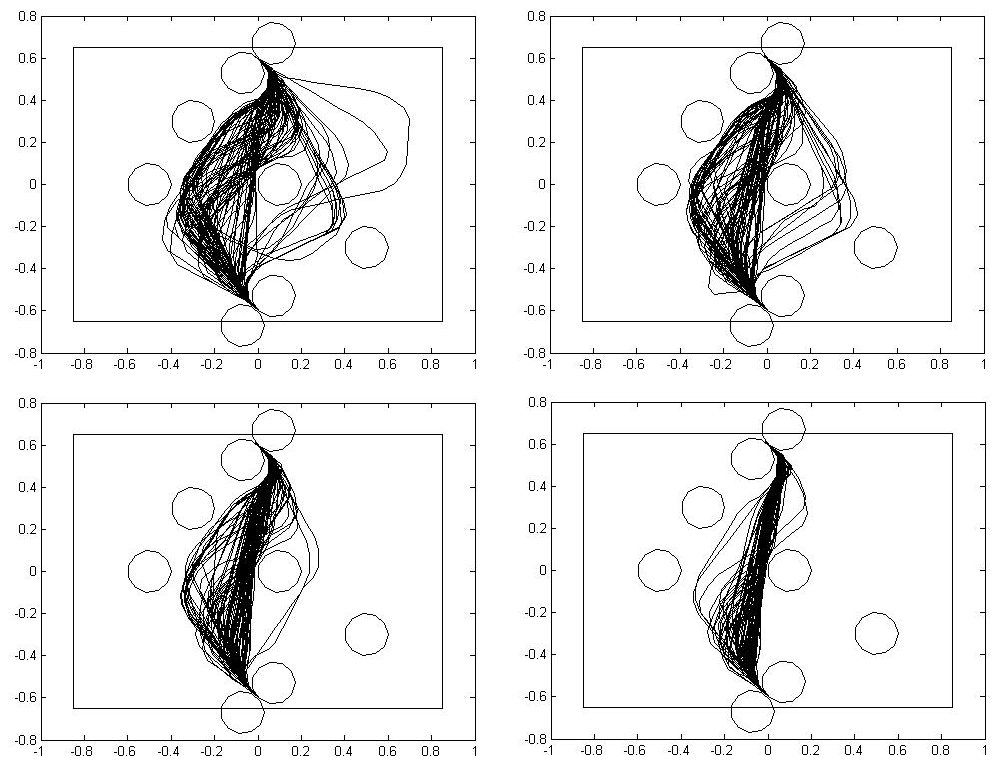
\includegraphics[width=1\textwidth]{figures/allsim.png}
    \vspace{0pt}\\
\end{tabular}

%\begin{figure}
%    \label{fig: rrtsim}
%	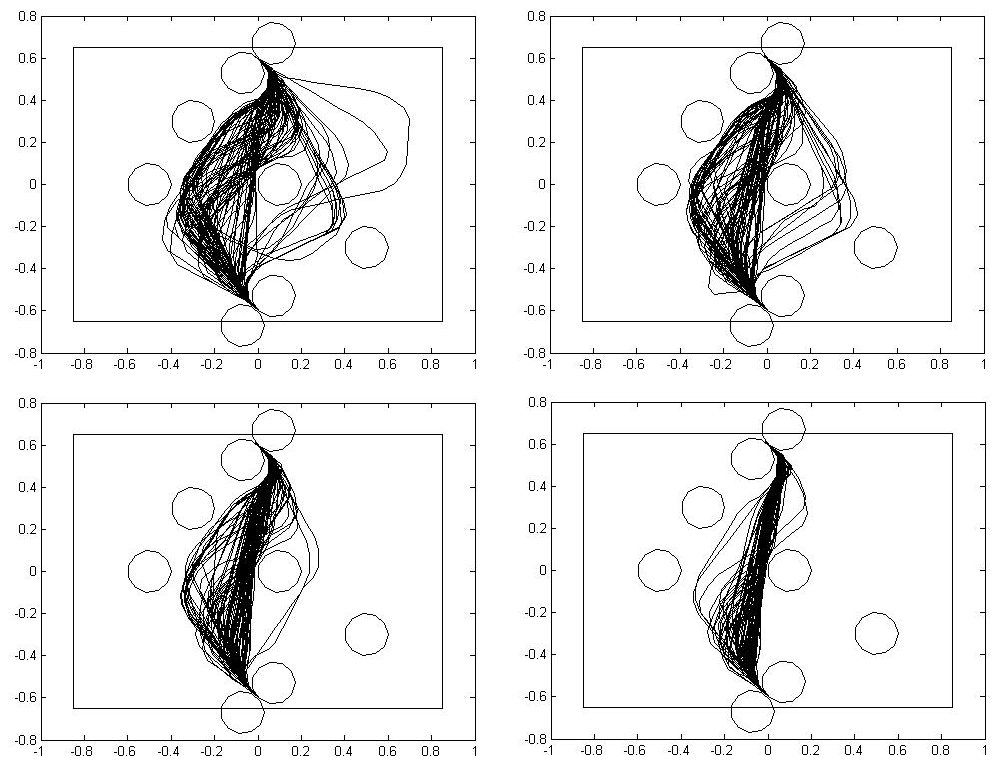
\includegraphics[width=1\textwidth]{figures/allsim.png}
%   	\caption{De esquerda para direita, cima pra baixo: 5, 10, 25 e 100 iterações.}
%\end{figure}

% Na figura acima, pode-se observar a variança nos caminhos. De esquerda para direita, cima pra baixo: 5, 10, 25 e 100 iterações. Um número menor de iterações é mais rápido, porém existe uma probabilidade maior de se encontrar uma trajetória não ótima e distante da anterior. Diante disso, foi escolhido o número máximo de iterações que respeita o limite de tempo de 2 ms com alguma folga: 15 iterações, que fazem uma média de 1,7 ms.

% \subsection{Otimização com MILP}
% \subsubsection{Navegação sobre todo o campo}

% O método de otimização aplicado sobre todo o campo se mostrou muito lento. O GLPK testa todas as possibilidades de combinações para as variáveis binárias, o que representa uma complexidade de $O(2^n)$. Nessa forma, para cada obstáculo e para cada passo, existem duas variáveis binárias. Por exemplo, para um vetor $b$ com 5 variáveis, existem 32 passos possíveis. Para 5 obstáculos (situação real), existem 10 variáveis binárias. O total de variáveis é de $5 + 32*10 = 325$, o que torna o algoritmo inaplicável para a complexidade dada. O método foi descartado na fase de testes em cenário simples.

\subsubsection{Navegação por uma triangulação}

O segundo método, por outro lado, permite o trabalho do GLPK sem levar os obstáculos em consideração, pois ao respeitar o limite dos triângulos, respeita-se ao mesmo tempo a restrição dos obstáculos. Tendo apenas 5 variáveis binárias, a complexidade $O(2^n)$ é admissível. No entando, ao se dividir o problema em triângulos e montar um algoritmo que resolve a transição por um triângulo, o algoritmo passou a não respeitar possíveis restrições do próximo triângulo enquanto soluciona o atual.

Por exemplo, foi usado para testes um gerador de situações aleatórias, que posiciona 5 obstáculos (três adversários e dois aliados) no campo. O otimizador leva o robô ao próximo triângulo com sucesso, entrentanto ele chega com uma posição e direção desfavoráveis para a solução do próximo. Em mais da metade dos testes aleatórios, o otimizador GLPK acusou erro de equação sem solução para algum trecho.

Tentar expandir as restrições do triângulo seguinte para o atual acabou por exigir uma quantidade maior de equações de restrição, o que desacelerou o algoritmo e acabou por não conseguir resolver inteiramente o problema. Diante dessa situação, este método também foi descartado ainda na fase de testes em cenário simples.

\section{Conclusões}

O projeto de Iniciação Científica apresentou bons resultados, especialmente quanto à vitória da equipe do ITA até às quartas de final da CBR 2017, rendendo o sétimo lugar à equipe dentre mais de 25 equipes participantes. Além do fato de que a ITAndroids conquistou o primeiro lugar na competição nacional de VSSS Copa Turing 2017, que ocorreu no final de setembro de 2017.

Do ponto de vista técnico, o uso do algoritmo da Behavior Tree, já consagrado e usado por times de nível mundial, se mostrou factível e funcional em partidas reais de competições. Contudo, problemas como pouca escalabilidade e pouca reutilizabilidade se mostraram presentes na estratégia desenvolvida. Isso significa que mudanças ainda deverão ser feitas nas BT, principalmente a respeito do uso de mais nós do tipo paralelo para remover esses problemas citados.

\section{Agradecimentos}

\begin{itemize}
\item Ao CNPq, pelo apoio financeiro e motivacional.
\item À ITAndroids, equipe que representa o ITA na competição da LARC/CBR, pela ideia do projeto, pela disponibilidade do robô real para implementação e oportunidade de aplicação dos métodos estudados.
\item Ao professor doutor Paulo Marcelo Tasinaffo, meu orientador, e ao professor doutor Marcos Ricardo de Omena Máximo, co-orientador, ambos da Divisão da Ciência da Computação do ITA, pelo apoio nos estudos e no desenvolvimento do projeto.

\end{itemize}

\section{Bibliografia}

\printbibliography


\end{document}